%%%%%%%%%%%%%%%%%%%%%%%%%%%%%%%%%%%%%%%%%%%%%%%%%%%%%%%%%%%%%%%%%%%%%
% Imperial College
\documentclass[a4paper,11pt,twoside]{article}
\usepackage[left=2.5cm,right=2cm,top=2cm,bottom=2cm]{geometry}

%%%%%%%%%%%%%%%%%%%%%%%%%%%%%%%%%%%%%%%%%%%%%%%%%%%%%%%%%%%%%%%%%%%%%
% Paragraph
\usepackage[parfill]{parskip}

% Images
\usepackage{graphicx}

% URLs
\usepackage{hyperref}

% Maths
\usepackage{amsmath}

%%%%%%%%%%%%%%%%%%%%%%%%%%%%%%%%%%%%%%%%%%%%%%%%%%%%%%%%%%%%%%%%%%%%%
\begin{document}
\title{Testing Numerical Methods for Integrating Systems of ODEs using 
the Case of a Pendulum}
\author{Dakshina Scott}
\date{\today}
\maketitle

%%%%%%%%%%%%%%%%%%%%%%%%%%%%%%%%%%%%%%%%%%%%%%%%%%%%%%%%%%%%%%%%%%%%%
\begin{abstract}

\end{abstract}

%%%%%%%%%%%%%%%%%%%%%%%%%%%%%%%%%%%%%%%%%%%%%%%%%%%%%%%%%%%%%%%%%%%%%

\tableofcontents

%%%%%%%%%%%%%%%%%%%%%%%%%%%%%%%%%%%%%%%%%%%%%%%%%%%%%%%%%%%%%%%%%%%%%

\section{Introduction}

In this investigation we begin by using the dynamics of a simple 
pendulum to examine three methods of numerical integration - Euler's
method, the leapfrog method, and the fourth-order Runge-Kutta 
method (RK4). Based on stability analyses of each method the most 
appropriate is then chosen for use on a double pendulum. Due to the 
chaotic nature of a double pendulum system it is important that 
the chosen method is the most stable. 

The equation of motion for a simple pendulum of mass \(m\) and length 
\(l\), at angle \(\theta\) from the vertical is given by

\begin{equation}
	\label{eq:eom}
	ml\frac{d^{2} \theta}{d t^{2}} = - mg\sin{\theta} - \gamma\frac{d \theta}{d t},
\end{equation}

where \(\gamma\) is a damping coefficient.

In natural units this becomes 

\begin{equation}
	\label{eq:natu}
	\frac{d^{2} \theta}{d \tau^{2}} = - mg\sin(\theta) - \frac{\gamma}{m\sqrt{gl}},
\end{equation}

where \(\tau\) is in units of \(\sqrt{\frac{l}{g}}\).

In order to numerically solve equation~\ref{eq:natu}, we first must 
separate it into a system of two coupled first-order differential 
equations:

\begin{equation}
	\label{dtheta}
	\frac{d \theta}{d \tau} = \omega,
\end{equation}

and

\begin{equation}
	\label{domega}
	\frac{d \omega}{d \tau} = -\theta - G\omega,
\end{equation}

where we have taken the small angle approximation for \(\sin\theta\) 
and G is a constant related to the damping coefficient by
\(G = \frac{\gamma}{m\sqrt{lg}}\).

While it is possible to determine the stability conditions for Euler's
method analytically (is it for others??? - e.g. where), in the case of leapfrog and RK4 
we analyse the stability by other means.

In any closed physical system, we know that energy is 
conserved - i.e. the total energy of the system remains 
constant over time. However, when using numerical methods we don't have 
an exact model for a sytem - only approximations. By looking at 
how the energy of our model deviates from being constant, we can see 
how the error in the method changes over time - an increasing error 
(or increasing deviations from constant energy) implies instablity, while a constant 
or decreasing error implies a stable method (for a given step size).

Here we first determine the stability of Euler's method analytically. 
We then compare this to the result of using the energy of the system 
to find stability conditions - this should confirm both that the program 
for Euler's method is working and that energy analysis is an effective 
way to assess stability.

Next we apply the energy analysis to the other two methods in order to 
see how their stability depends on step size. This will allow us to choose 
an appropriate method for the double pendulum.

\section{Euler's Method}
Euler's method is the simplest method for numerically integrating a 
system of ODEs with given initial conditions. In this method the value 
of the derivative at an initial point is used to estimate a new y-value 
after a small step forward in the x-axis. This apprach works well on
functions with constant or slowly changing gradients, but for a 
a function with a rapidly changing gradient (e.g. for an oscilating 
pendulum) one would not expect this to give very good estimates.

%\begin{figure}{htb}
%	\centering
%	\includegraphics[width=0.8\textwidth]{euler_example.png}
%	\caption{For a non-linear function, Euler's method is not 
%		very accurate. The greater the change in gradient within the chosen 
%	step size, the larger the truncation error is for that step.}
%	\label{fig:eulerexample}
%\end{figure}

While a smaller step size does generally improve accuracy, there is 
a limit to this, beyond which the local error will be dominated by 
another error - the round-off error. A computer can only store a 
finite number of significant figures, and when it reaches this limit 
it rounds the number being stored. As a result of this, for a variable 
stored as type double the smallest useful step size is \(~10^{-8}\).

First by trial and error we find that the undamped case is unstable 
even for the minimum-error case.
In the undamped case even for step size as small as h = 0.00001, 
a graph of energy against time clearly shows increasing oscillation 
amplitudes.
FIGURE??? - do h = 0.00000001 overnight?

In the damped case, with \(\gamma = 0.2\), we again look for a 
stability condition by trial and error. Below is a graph showing the 
energy against time for various step sizes, including the one which, by
eye, appears to be the limiting case for stability. 

\begin{figure}{htb}
	\centering
	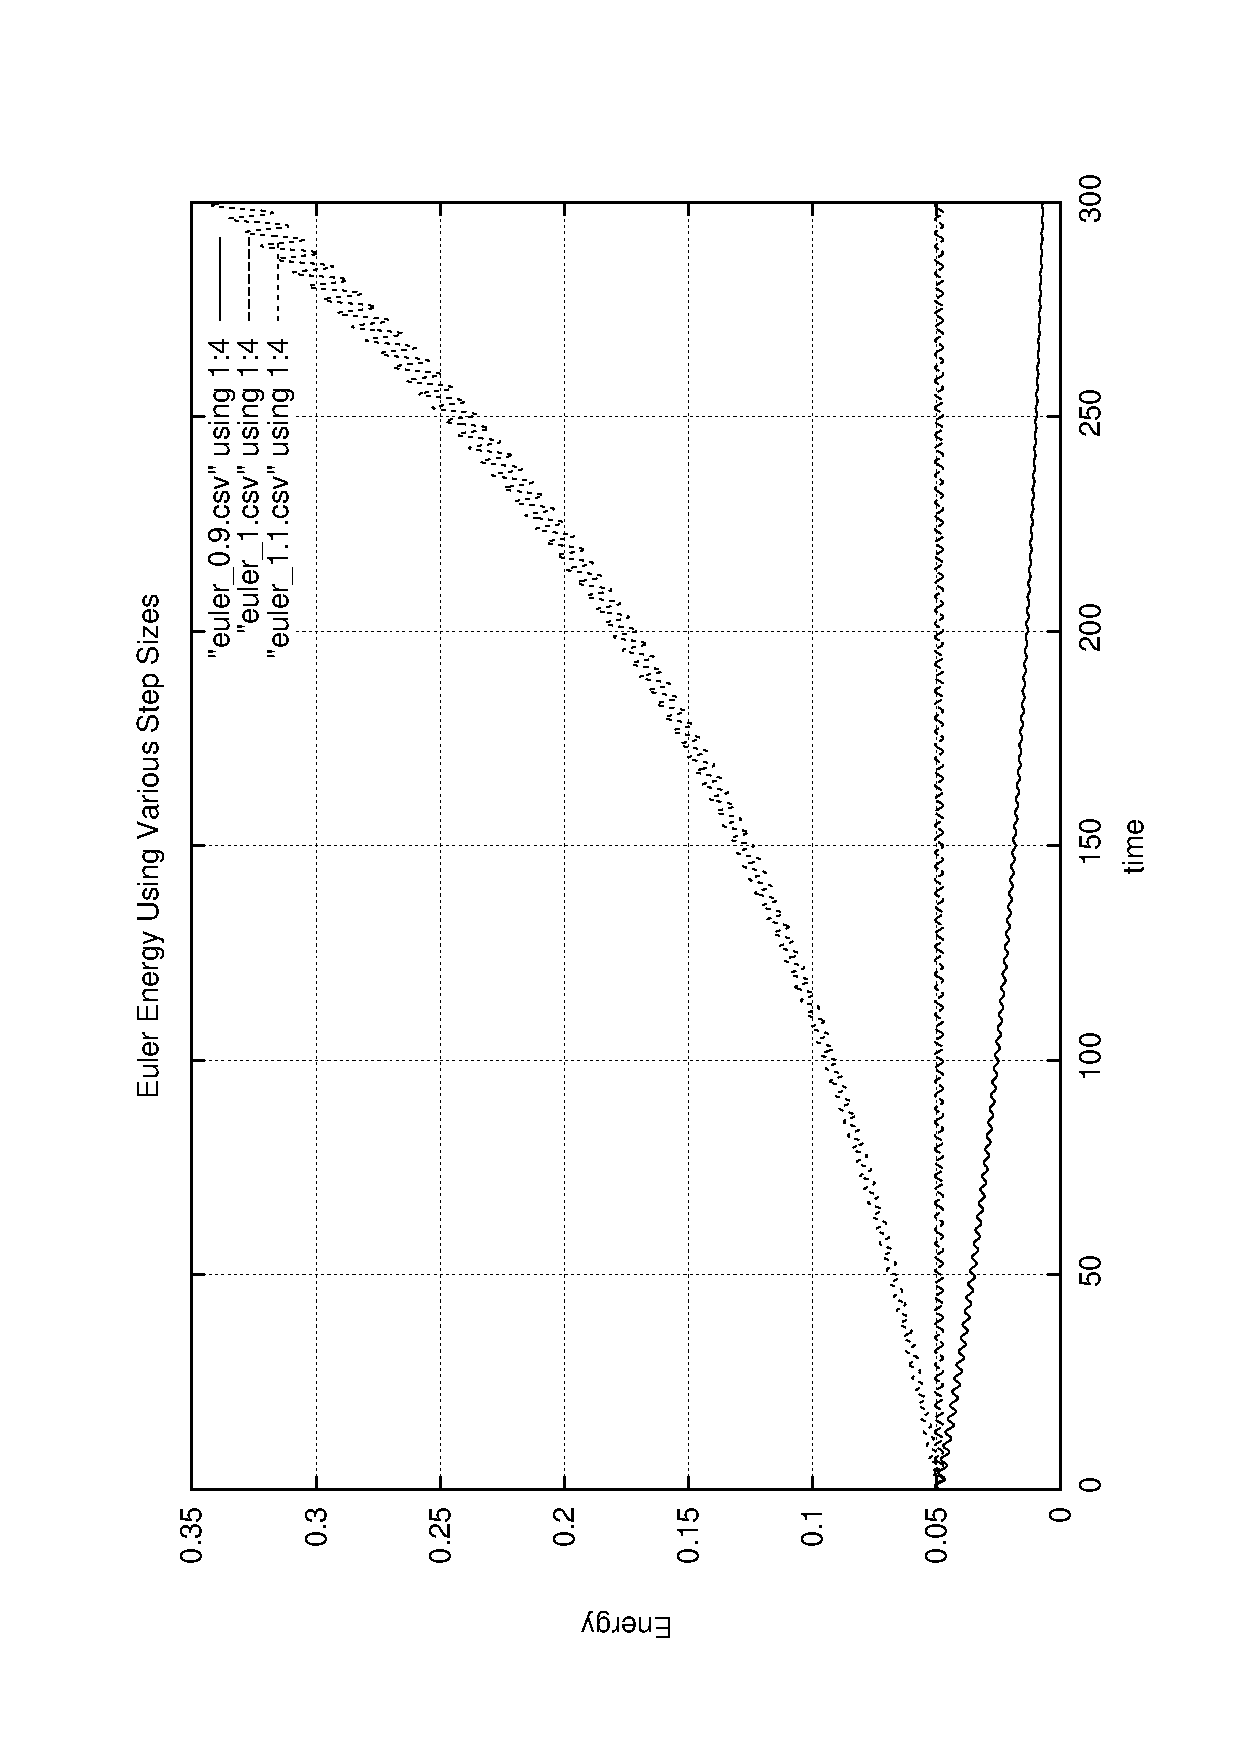
\includegraphics[width=0.8\textwidth]{euler_energies.png}
	\caption{Energy for different step sizes dt, with \(\gamma = 0.2\). 
		Step size of dt = 0.2 looks like a good guess 
		for the limiting value for stability. Units aren't included 
		as we're interested in relative changes in energy.}
	\label{fig:eulercond}
\end{figure}

Using the characteristic equation of the update matrix for our coupled 
system we can find it's eigenvalues \(\lambda^{1}\) and \(\lambda^{2}\). 
It can be shown that for \(|\lambda^{i}|^{2} \leq 1\) the system is stable.
(SOURCE???). For Euler's method this results in the stabilty condition

\begin{equation}
	\label{eq:stab}
	h \leq G
\end{equation}

where \(h\) is the step size.
From this it's clear that for an undamped system (in which \(G=0\))
Euler's method is always unstable, as the step size is always positive.

%%%%%%%%%%%%%%%%%%%%%%%%%%%%%%%%%%%%%%%%%%%%%%%%%%%%%%%%%%%%%%%%%%%%%
\begin{thebibliography}{20}

bibitem{eulerexample}
Paul's Online Math Notes, 2012. [online] Available at \url{http://tutorial.math.lamar.edu/Classes/DE/EulersMethod.asp}
[Accessed 8 November 2012].

\end{thebibliography}

\end{document}

